\documentclass[conference]{IEEEtran}
\IEEEoverridecommandlockouts

\usepackage{cite}
\usepackage{amsmath,amssymb,amsfonts}
\usepackage{graphicx}
\usepackage{textcomp}
\usepackage{xcolor}
\usepackage{booktabs}
\usepackage{array}

\def\BibTeX{{\rm B\kern-.05em{\sc i\kern-.025em b}\kern-.08em
    T\kern-.1667em\lower.7ex\hbox{E}\kern-.125emX}}

\begin{document}

\title{Validator-Guided LLM Lowering from C Constructs to LLVM Intermediate Representation}
\author{

\IEEEauthorblockN{Varun Gowda R}
\IEEEauthorblockA{
\textit{Department of Computer Science and Engineering} \\
\textit{RV College of Engineering} \\
Bengaluru, India \\
varungowdar.cs23@rvce.edu.in
}
\and
\IEEEauthorblockN{Vishal K Bhat}
\IEEEauthorblockA{
\textit{Department of Computer Science and Engineering} \\
\textit{RV College of Engineering} \\
Bengaluru, India \\
vishalkbhat.cs23@rvce.edu.in
}
\and
\IEEEauthorblockN{Deepika Dash}
\IEEEauthorblockA{
\textit{Assistant Professor} \\
Department of Computer Science and Engineering \\
\textit{RV College of Engineering} \\
Bengaluru, India \\
deepikadash@rvce.edu.in
}

}

\maketitle

\begin{abstract}
Lowering high-level source programs to compiler intermediate representation requires exact handling of types, static single assignment form, and control-flow structure. This paper studies whether large language models can assist in translating a controlled subset of C programs into LLVM intermediate representation. We evaluate four instruction-tuned models across 15 C constructs, six construct levels, and two prompting strategies, producing 118 generation attempts. A custom validator checks syntax, static single assignment discipline, type consistency, control flow, and semantic patterns; failed outputs are further processed by an iterative repair loop. The results show that 89.8 percent of generated intermediate representations pass validation, with arithmetic and function-call constructs reaching 100 percent validity. The strongest model, Llama-3.3-70B, validates all generated outputs, while control-flow constructs remain the main source of errors. Basic prompting outperforms chain-of-thought prompting by 10.5 percentage points. The repair loop successfully repairs 7 of 8 failed constructs and reduces total validation errors from 11 to 1. These results suggest that language models are promising assistants for compiler lowering when paired with deterministic validation and repair.
\end{abstract}

\begin{IEEEkeywords}
compiler lowering, LLVM IR, large language models, program repair, validation, static single assignment
\end{IEEEkeywords}

\section{Introduction}
Compiler frontends translate source-language constructs into intermediate representation (IR), where later optimization and code-generation passes operate. This lowering step is precise: generated LLVM IR must preserve source semantics while satisfying structural requirements such as explicit basic blocks, typed instructions, terminators, and static single assignment (SSA) form. A lowering error is not merely a formatting issue; it can produce invalid code, incorrect control flow, or a silently wrong computation.

Large language models (LLMs) have demonstrated strong code-generation ability, but compiler IR occupies an unusual point in the code-generation spectrum. It is textual and regular enough for language models to emit, yet strict enough that small mistakes can invalidate the whole program. Prior work has examined LLMs for compiler optimization \cite{cummins2023compiler}, compiler-feedback loops \cite{grubisic2024feedback}, IR understanding \cite{jiang2025ir}, and IR-enhanced multilingual code generation \cite{paul2024ircoder}. This paper focuses on the forward lowering problem: given a small C construct, can an LLM generate valid LLVM IR?

We make three contributions. First, we define a benchmark of 15 C constructs spanning arithmetic, control flow, functions, memory, aggregates, and composite programs. Second, we evaluate four open instruction-tuned LLMs under basic and chain-of-thought prompting using a five-pass LLVM IR validator. Third, we measure the effectiveness of validator-guided repair on failed outputs.

\section{Problem Formulation}
Given a source construct $S$ in a restricted C subset, the task is to generate LLVM IR $I$ such that $I$ is syntactically well formed, compilable, structurally faithful to the expected control-flow graph, and semantically consistent with a reference lowering.

The experiment asks four research questions:

\begin{itemize}
\item RQ1: Can LLMs map simple high-level C constructs into valid LLVM IR?
\item RQ2: Do LLMs preserve control-flow and data-flow structure during lowering?
\item RQ3: How do model choice and prompting strategy affect validity?
\item RQ4: Can validator-guided repair improve failed generations?
\end{itemize}

\section{Methodology}
\subsection{Source Construct Set}
The source language subset contains 15 C constructs grouped into six levels. The levels are designed to increase in compiler complexity rather than source-code length. Table~\ref{tab:constructs} summarizes the benchmark.

\begin{table}[htbp]
\caption{Source Construct Levels}
\label{tab:constructs}
\centering
\begin{tabular}{@{}clcl@{}}
\toprule
Level & Category & Count & Main IR Features\\
\midrule
L1 & Arithmetic and assignment & 4 & Integer, float, bitwise ops\\
L2 & Control flow & 4 & Branches, loops, phi nodes\\
L3 & Functions and calls & 2 & Calls and recursion\\
L4 & Pointers and memory & 2 & Load, store, indexing\\
L5 & Structs and aggregates & 1 & Struct type and field access\\
L6 & Composite programs & 2 & Combined memory and control flow\\
\bottomrule
\end{tabular}
\end{table}

\subsection{Models and Prompting}
The evaluation uses four instruction-tuned models: Qwen2.5-Coder-32B, Qwen2.5-72B, Llama-3.3-70B, and Llama-3.1-8B. Each construct is tested with two prompting strategies. The basic strategy asks directly for LLVM IR. The chain-of-thought strategy asks the model to reason through signature, control flow, SSA values, and block structure before producing IR. In total, the pipeline records 118 generation attempts.

\subsection{Validation Pipeline}
Each generated IR output is processed by a five-pass validator. The passes check structural syntax, SSA correctness, type use, control-flow well-formedness, and semantic correspondence against expected patterns. The validator reports whether a generation is valid, compilable, and structurally correct, along with detailed errors and warnings.

Failures are assigned to a taxonomy with five major classes: structural or syntactic failures, control-flow failures, type-system failures, semantic or functional failures, and scale or context failures. The observed failures in this experiment fall into three of these classes.

\subsection{Repair Loop}
Failed outputs are passed to an iterative repair loop. At each iteration, the repair component receives the original source, generated IR, reference information, and validator feedback. The repaired IR is validated again, and the process stops when validation succeeds or the iteration budget is exhausted. Repair is evaluated by success rate, error reduction, iteration count, and repair time.

\section{Experimental Results}
\subsection{Overall Validity}
Across 118 generation attempts, 106 outputs are valid and 110 are compilable, yielding an overall validation rate of 89.8\% and a compilability rate of 93.2\%. The gap between compilability and validity shows that some IR can compile while still violating expected structure or semantics.

\subsection{Model-Level Performance}
Llama-3.3-70B achieves 100.0\% validity across 30 generations. Qwen2.5-Coder-32B follows with 93.3\%, Llama-3.1-8B reaches 89.7\%, and Qwen2.5-72B reaches 75.9\%. The weaker aggregate scores are concentrated in control-flow-heavy and composite constructs rather than uniformly distributed across the benchmark. Table~\ref{tab:model-results} reports overall model performance, while Table~\ref{tab:construct-difficulty} lists the most difficult constructs and preserves the construct-level signal without relying on a heatmap.

\begin{table}[htbp]
\caption{Model Performance}
\label{tab:model-results}
\centering
\begin{tabular}{@{}lccc@{}}
\toprule
Model & Valid & Compilable & Avg. Time\\
 & (\%) & (\%) & (s)\\
\midrule
Llama-3.3-70B & 100.0 & 100.0 & 1.53\\
Qwen2.5-Coder-32B & 93.3 & 100.0 & 3.67\\
Llama-3.1-8B & 89.7 & 89.7 & 0.33\\
Qwen2.5-72B & 75.9 & 82.8 & 22.80\\
\bottomrule
\end{tabular}
\end{table}

The results indicate that larger parameter count alone does not predict lowering quality: Qwen2.5-72B is slower and less valid than the smaller Qwen coder model. Fig.~\ref{fig:latency-validity} visualizes this latency-validity tradeoff using raw timing data from the generation logs.

\begin{figure}[htbp]
\centering
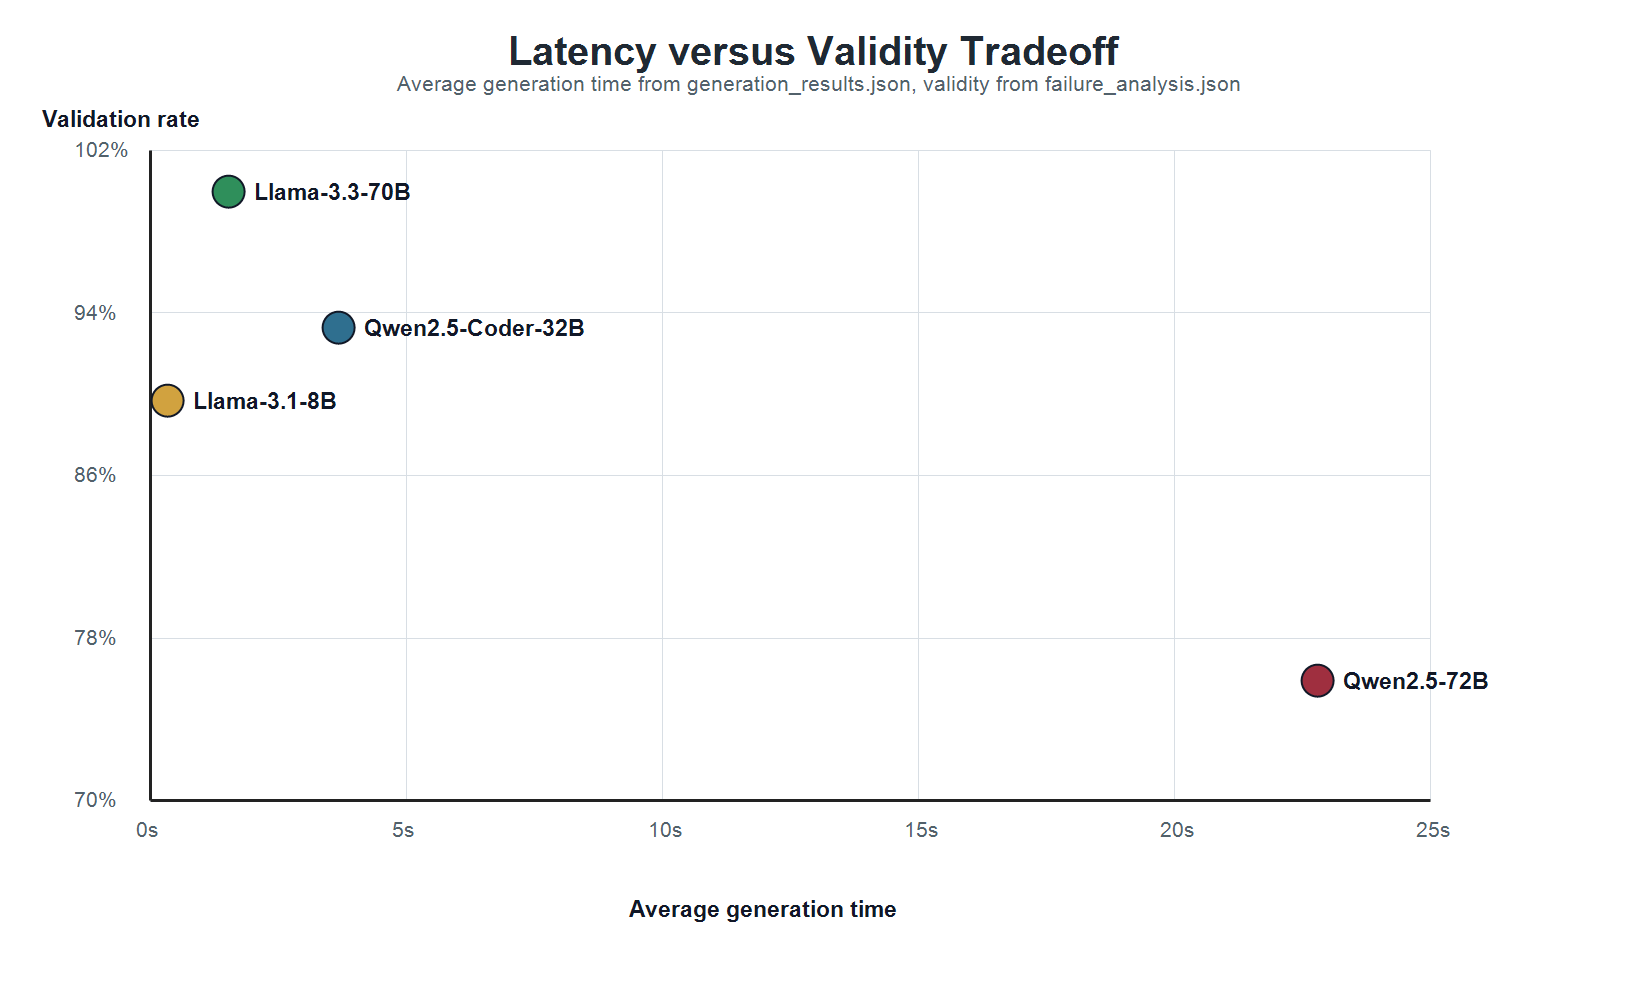
\includegraphics[width=\columnwidth]{results/figures/latency_validity_scatter.png}
\caption{Average generation latency versus validation rate. The fastest model is not the most valid, and the slowest model is not the most reliable.}
\label{fig:latency-validity}
\end{figure}

\subsection{Construct-Level Performance}
L1 arithmetic and L3 function constructs achieve 100.0\% validity. L2 control flow validates at 84.4\%, L4 memory at 86.7\%, L5 aggregates at 87.5\%, and L6 composite constructs at 75.0\%. This pattern supports the hypothesis that LLMs can lower local expressions reliably but struggle when values must be threaded across multiple blocks. Table~\ref{tab:construct-difficulty} shows the most informative construct-level rates, and Fig.~\ref{fig:complexity-ratio} adds a structural view by comparing generated IR size against reference IR size.

\begin{table}[htbp]
\caption{Most Informative Construct-Level Validity Results}
\label{tab:construct-difficulty}
\centering
\begin{tabular}{@{}llc@{}}
\toprule
Construct & Category & Valid (\%)\\
\midrule
Simple Addition & Arithmetic & 100.0\\
Floating Point Arithmetic & Arithmetic & 100.0\\
Function Call & Functions & 100.0\\
Recursive Function & Functions & 100.0\\
If-Else Branch & Control flow & 75.0\\
Array Sum & Memory & 75.0\\
Struct Field Access & Aggregates & 87.5\\
Bubble Sort & Composite & 62.5\\
Linked List Length & Composite & 87.5\\
\bottomrule
\end{tabular}
\end{table}

\begin{figure}[htbp]
\centering
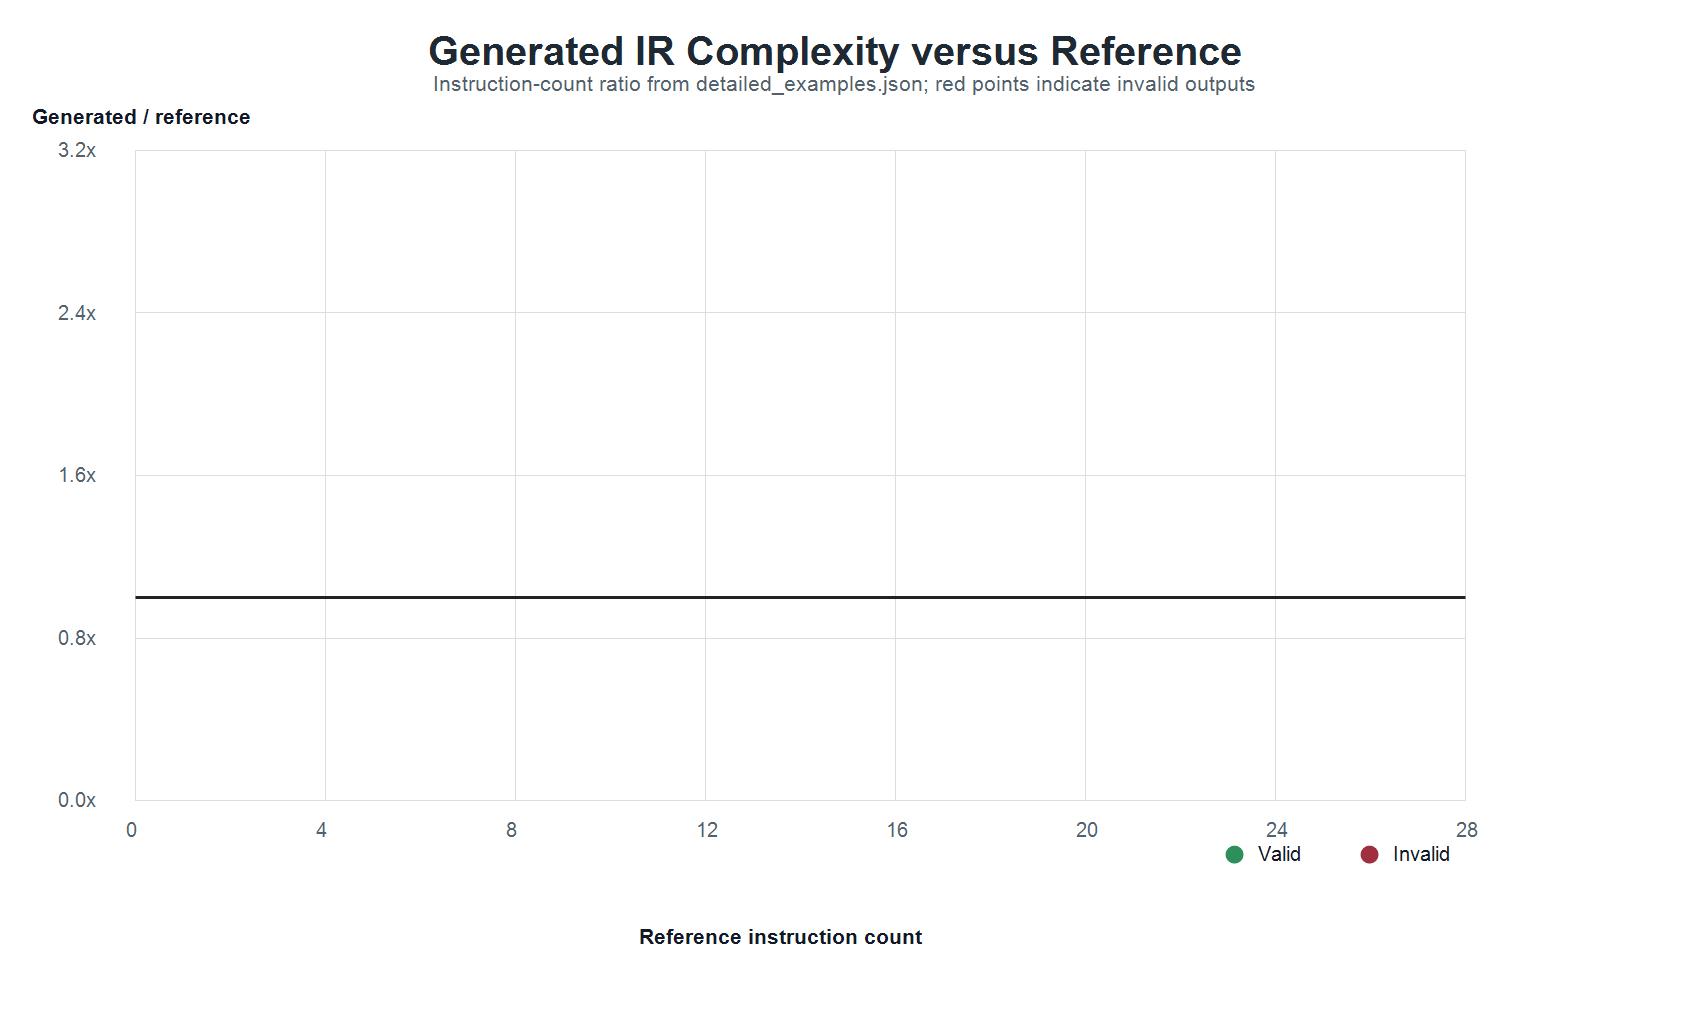
\includegraphics[width=\columnwidth]{results/figures/ir_complexity_ratio_scatter.png}
\caption{Generated IR complexity relative to reference IR. Invalid outputs tend to appear among examples whose generated IR is inflated relative to the reference lowering.}
\label{fig:complexity-ratio}
\end{figure}

\subsection{Prompting Strategy}
Basic prompting validates 57 of 60 generations, or 95.0\%. Chain-of-thought prompting validates 49 of 58 generations, or 84.5\%. The lower chain-of-thought score is consistent with a practical failure mode: verbose responses are more likely to mix explanatory text, overfit to plausible patterns, or emit control-flow structures that appear reasoned but fail validator checks. Table~\ref{tab:prompt-results} summarizes the aggregate comparison, and Fig.~\ref{fig:verbosity} shows that chain-of-thought prompting systematically expands response length relative to the extracted IR artifact.

\begin{table}[htbp]
\caption{Prompting Strategy Comparison}
\label{tab:prompt-results}
\centering
\begin{tabular}{@{}lcc@{}}
\toprule
Prompt strategy & Total & Valid (\%)\\
\midrule
Basic & 60 & 95.0\\
Chain-of-thought & 58 & 84.5\\
\bottomrule
\end{tabular}
\end{table}

\begin{figure}[htbp]
\centering
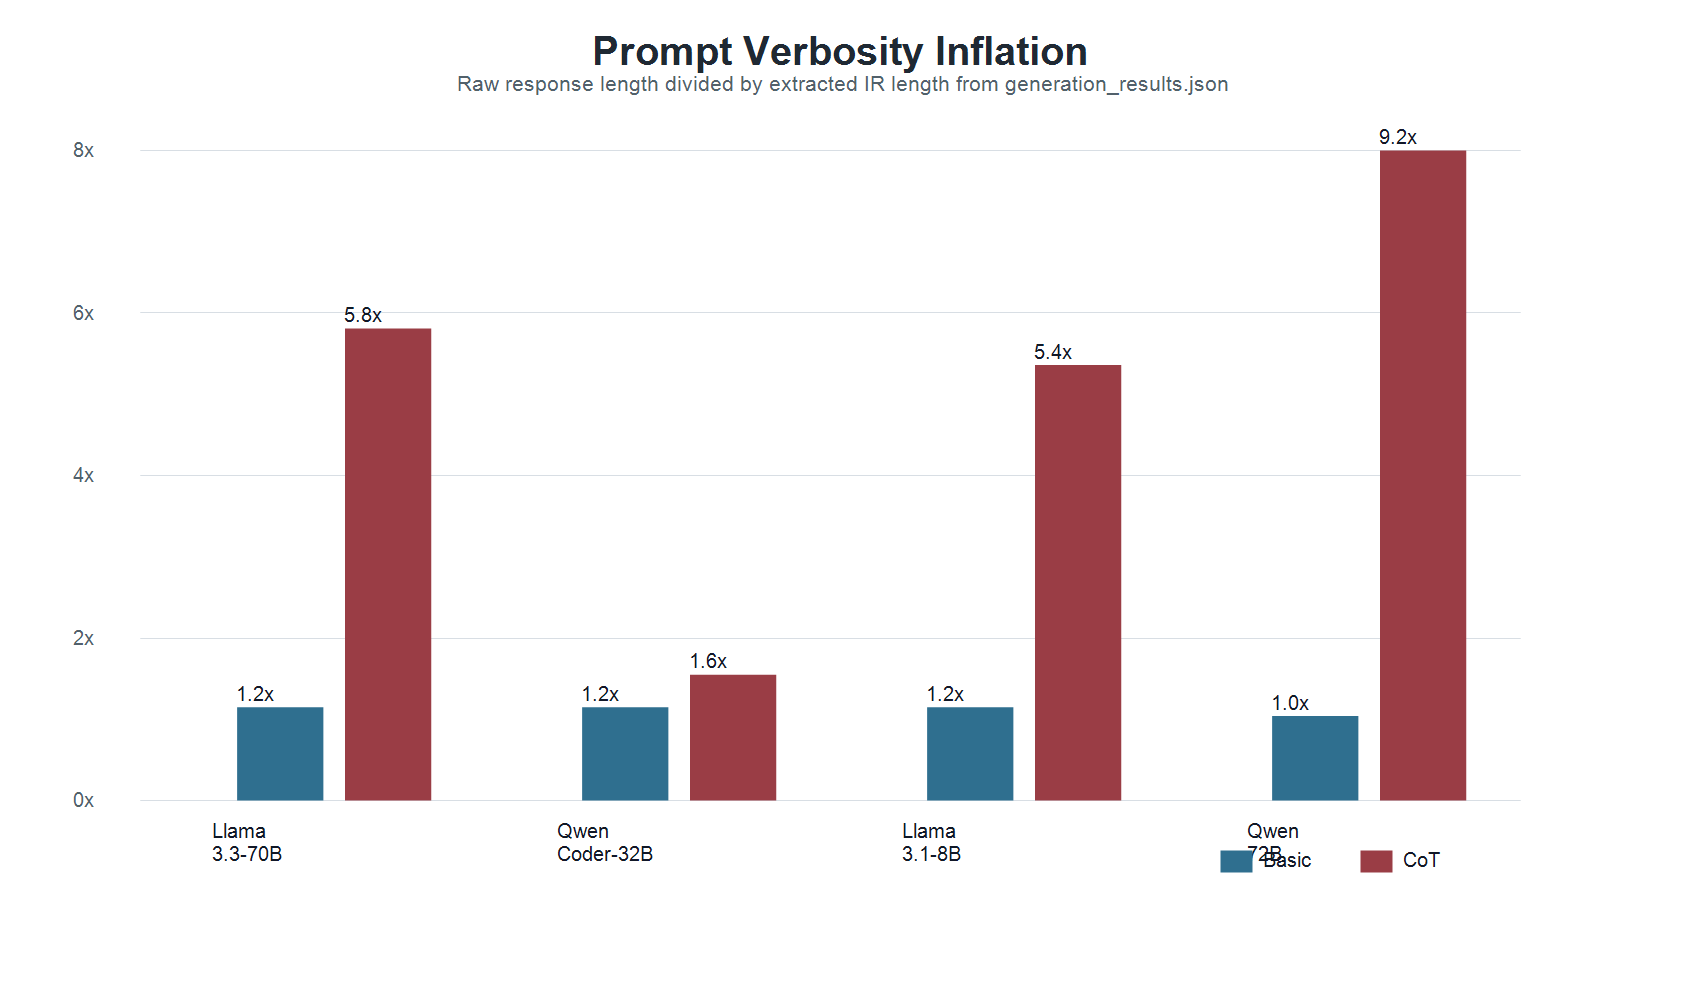
\includegraphics[width=\columnwidth]{results/figures/prompt_verbosity_inflation.png}
\caption{Prompt verbosity inflation computed as raw response length divided by extracted IR length. Chain-of-thought prompting often expands responses beyond the IR artifact itself.}
\label{fig:verbosity}
\end{figure}

\subsection{Failure Analysis}
The validator records 57 total failure instances. As shown in Fig.~\ref{fig:failure-pareto}, control-flow failures dominate with 38 instances, representing 66.7\% of all observed failures. Structural or syntactic failures account for 14 instances, and semantic or functional failures account for 5 instances.

\begin{figure}[htbp]
\centering
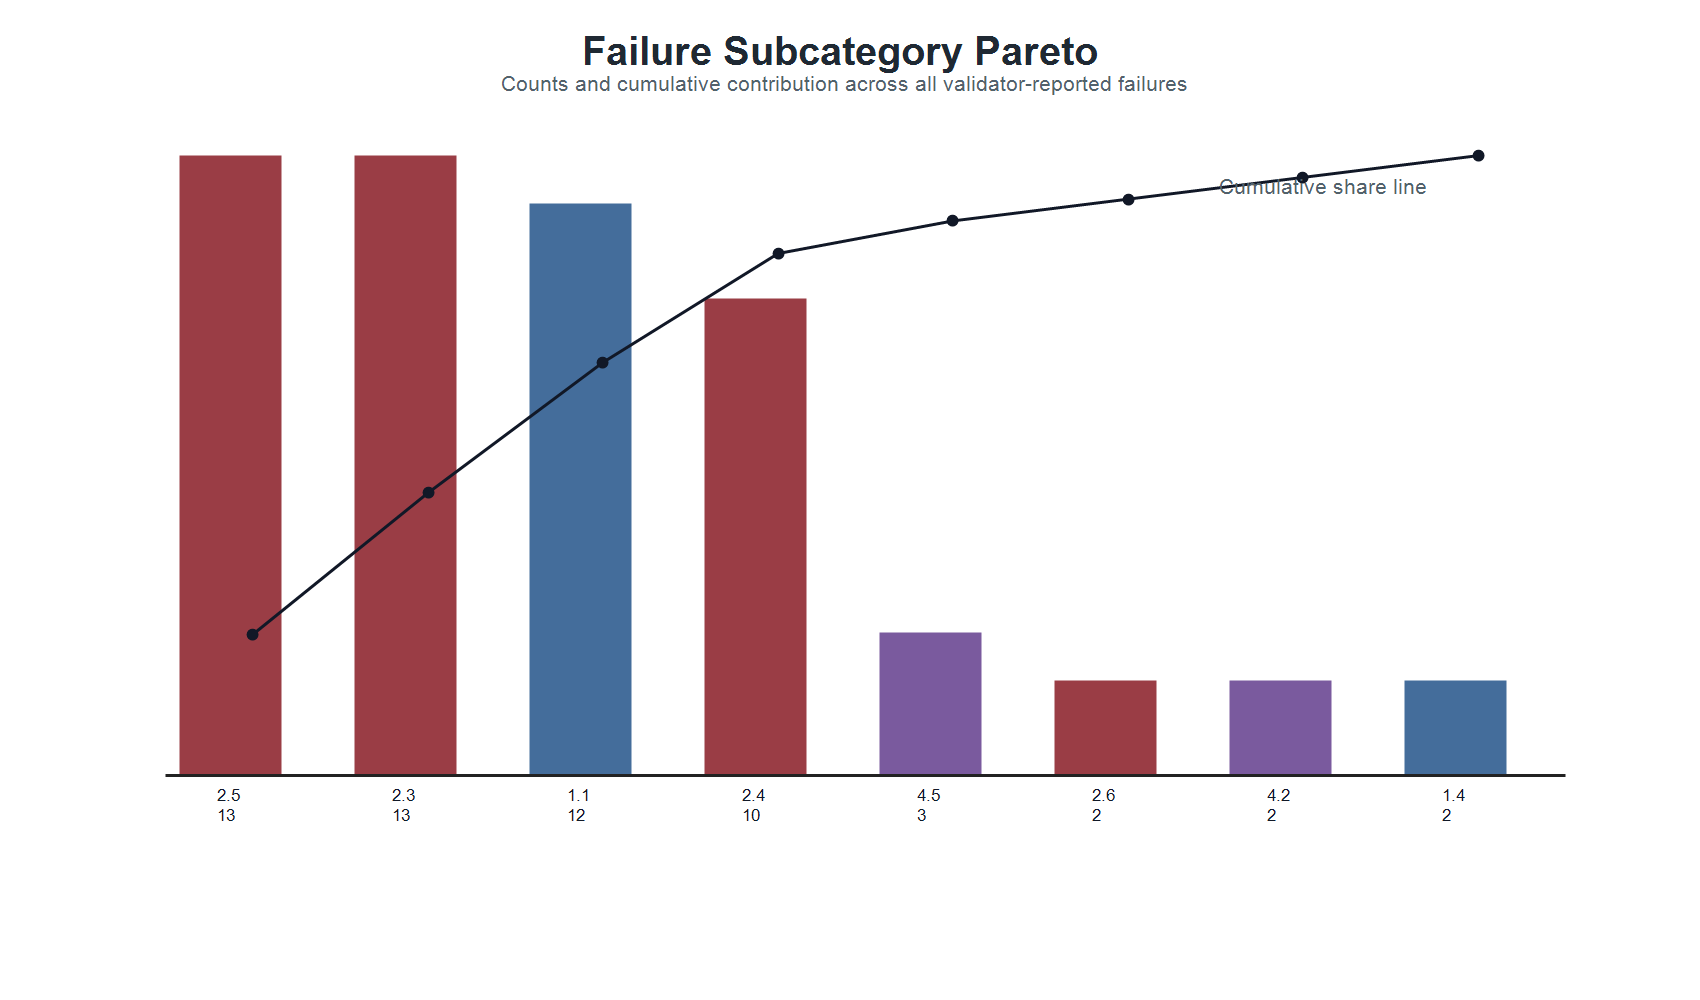
\includegraphics[width=\columnwidth]{results/figures/failure_subcategory_pareto.png}
\caption{Failure subcategory Pareto chart. Incorrect phi-node predecessors, unreachable or extra code paths, SSA violations, and loop approximation explain most of the observed failures.}
\label{fig:failure-pareto}
\end{figure}

The most frequent subcategories are incorrect phi-node predecessors and unreachable or extra code paths, each with 13 instances. SSA violations occur 12 times, and loop approximation occurs 10 times. These errors are compiler-specific: they are not simply natural-language misunderstandings, but violations of the invariants that make LLVM IR executable and analyzable.

\begin{figure}[htbp]
\centering
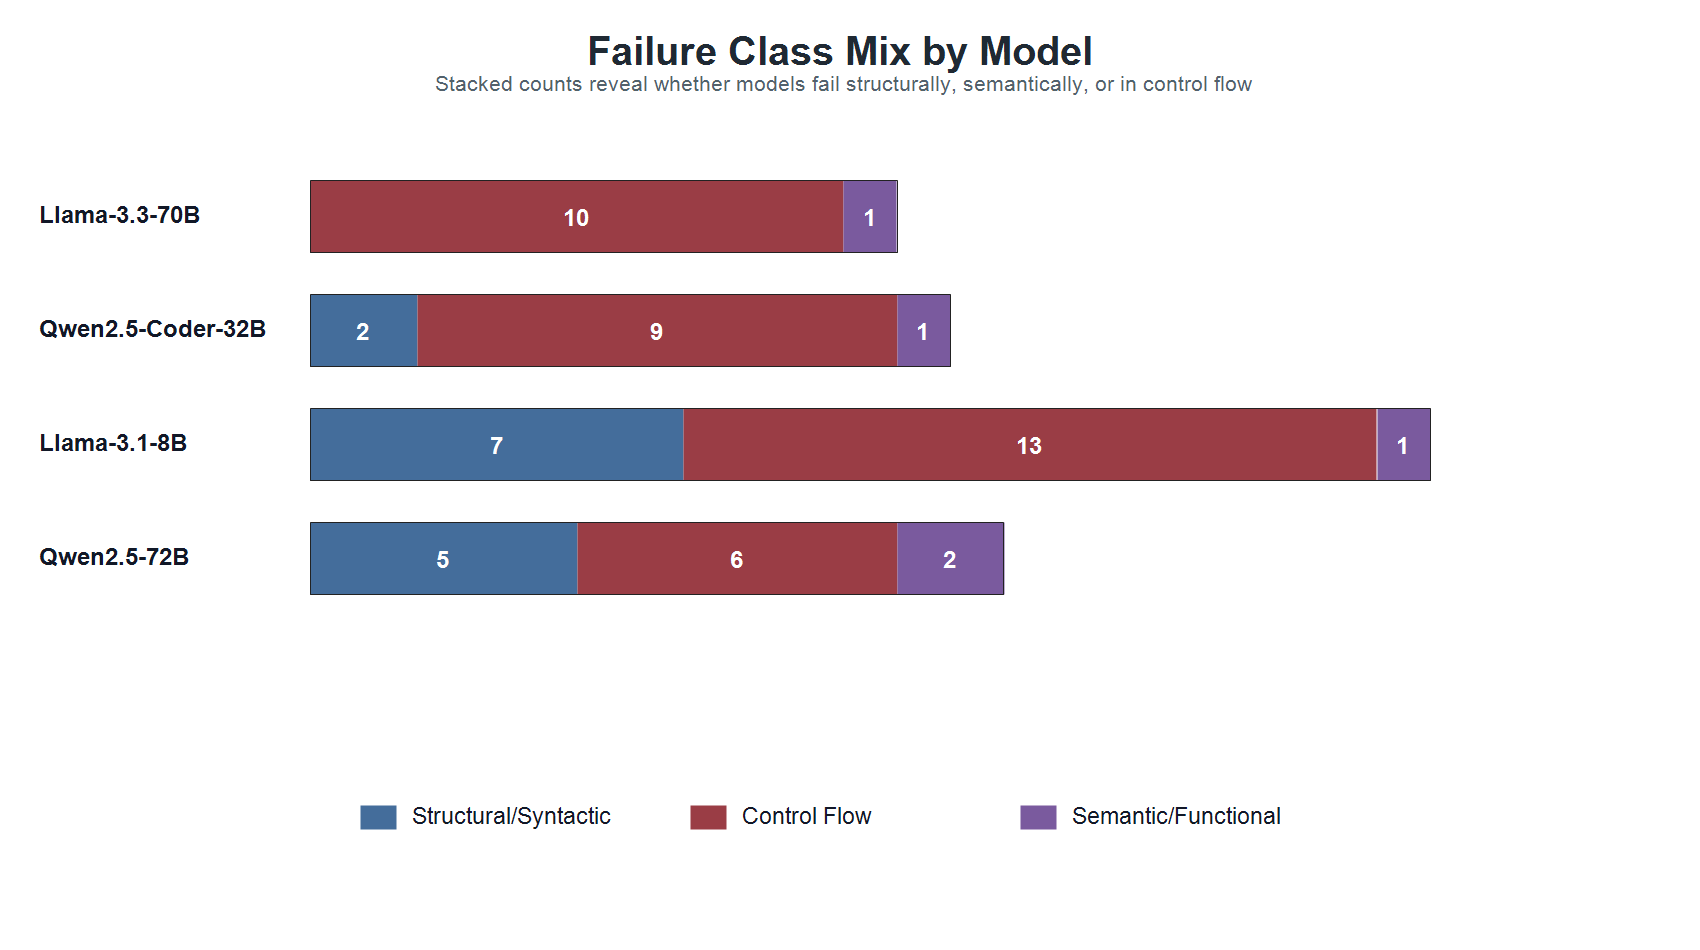
\includegraphics[width=\columnwidth]{results/figures/model_failure_class_stacked.png}
\caption{Failure-class mix by model. Control-flow errors dominate across models, while structural and semantic failures remain secondary but non-negligible.}
\label{fig:model-failure-mix}
\end{figure}

\subsection{Repair Effectiveness}
The repair loop is applied to 8 failed constructs. It succeeds on 7 of them, giving an 87.5\% repair success rate. Total validation errors fall from 11 to 1, a 90.9\% reduction. Repairs require 10 total iterations, with an average of 1.2 iterations per repair and 7.7 seconds per repair attempt. Fig.~\ref{fig:repair-trajectories} shows that most failed generations converge after one iteration, which suggests that validator feedback is specific enough to guide targeted fixes rather than repeated exploratory regeneration.

\begin{figure}[htbp]
\centering
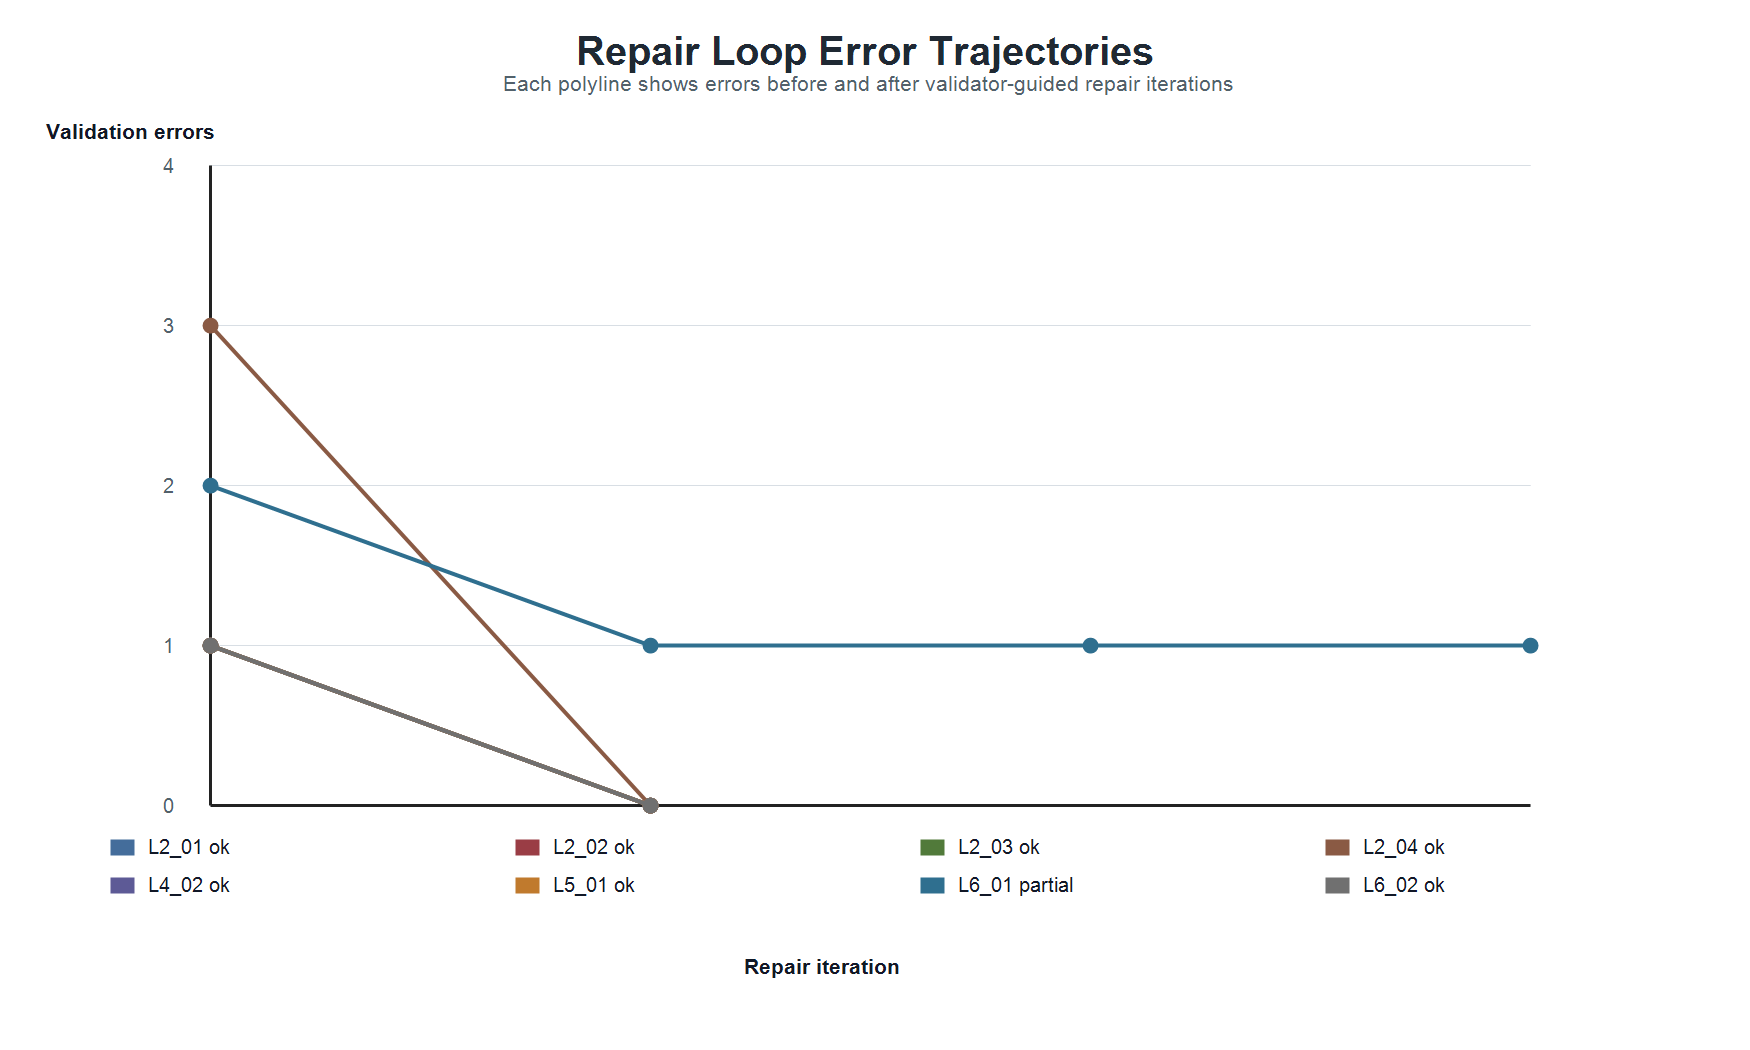
\includegraphics[width=\columnwidth]{results/figures/repair_error_trajectories.png}
\caption{Repair-loop error trajectories by construct. Most repairs converge to zero validation errors after one iteration, while one composite construct remains partially repaired.}
\label{fig:repair-trajectories}
\end{figure}

\section{Discussion}
The results suggest that LLM-based lowering is most reliable for expression-level and direct-call constructs. Arithmetic, bitwise operations, floating-point expressions, and simple calls map naturally to compact LLVM IR patterns. In these cases, the model needs to choose correct opcodes and preserve function signatures, but it does not need to construct complex control-flow graphs.

The frontier is control flow. Loops and nested branches require coordinated block labels, branch targets, phi-node incoming edges, and loop-carried values. A model can generate text that resembles LLVM IR while still assigning a phi predecessor to the wrong block or simplifying a loop into an invalid approximation. These failures explain why validation must be part of the architecture rather than a post-hoc grading step.

The prompt comparison is also notable. Chain-of-thought prompting often improves reasoning tasks, but here direct prompting performs better. LLVM IR generation benefits from concise outputs with little surrounding text. Asking the model to reason explicitly may increase the chance of extra prose, hallucinated intermediate assumptions, or unnecessarily elaborate block structure.

The repair results show the value of compiler-style feedback. Even when first-pass generation fails, validator diagnostics provide a concrete signal that can guide correction. The absence of repair regressions in the recorded statistics is encouraging, although the single unrepaired composite construct indicates that complex memory-and-control-flow interactions still require stronger repair strategies.

\section{Threats to Validity}
The benchmark uses a restricted C subset and 15 constructs, so the results should not be interpreted as full C frontend replacement. The reference IR patterns may favor common canonical lowerings, while alternative valid lowerings may be penalized if they differ structurally. The generation count is also not perfectly balanced across all model and prompt combinations because the recorded dataset contains 118 rather than 120 attempts. Finally, validation approximates semantic equivalence through structural and pattern checks; complete functional equivalence would require execution-based testing or formal equivalence checking.

\section{Conclusion}
This paper evaluated LLM-assisted lowering from C constructs to LLVM IR using four models, two prompting strategies, a custom validator, and an iterative repair loop. The main finding is that LLMs can generate valid IR for simple-to-moderate constructs at high rates, reaching 89.8\% overall validity and 100.0\% validity on arithmetic and function-call levels. However, control flow remains the main source of failures, especially phi-node and loop-structure errors. Basic prompting is more effective than chain-of-thought prompting for this task, and validator-guided repair substantially improves failed outputs. These findings support a hybrid architecture in which LLMs propose lowerings and deterministic compiler tools validate and repair them before use.

\section*{Acknowledgment}
The authors thank the Department of Computer Science and Engineering for supporting the compiler design laboratory work that motivated this study.

\begin{thebibliography}{00}
\bibitem{jiang2025ir} H. Jiang, J. Zhu, Y. Wan, B. Fang, H. Zhang, R. Jin, and Q. Guan, ``Can large language models understand intermediate representations?'' CoRR, abs/2502.06854, 2025.
\bibitem{cummins2023compiler} C. Cummins, V. Seeker, D. Grubisic, M. Elhoushi, Y. Liang, B. Roziere, J. Gehring, F. Gloeckle, K. M. Hazelwood, G. Synnaeve, and H. Leather, ``Large language models for compiler optimization,'' CoRR, abs/2309.07062, 2023.
\bibitem{grubisic2024feedback} D. Grubisic, C. Cummins, V. Seeker, and H. Leather, ``Compiler generated feedback for large language models,'' CoRR, abs/2403.14714, 2024.
\bibitem{islam2024eda} M. ul Islam, H. Sami, P.-E. Gaillardon, and V. Tenace, ``EDA-aware RTL generation with large language models,'' CoRR, abs/2412.04485, 2024.
\bibitem{paul2024ircoder} I. Paul, J. Luo, G. Glavas, and I. Gurevych, ``IRCoder: Intermediate representations make language models robust multilingual code generators,'' CoRR, abs/2403.03894, 2024.
\bibitem{llvm} C. Lattner and V. Adve, ``LLVM: A compilation framework for lifelong program analysis and transformation,'' in \textit{Proc. International Symposium on Code Generation and Optimization}, 2004, pp. 75--86.
\end{thebibliography}

\end{document}
